% !TEX TS-program = XeLaTeX
%!TEX encoding = UTF-8 Unicode
%==================================================
%      PREAMBOLO e DICHIARAZIONI INIZIALI
%==================================================
\documentclass[10pt,oneside,a4paper]{article}

\usepackage[utf8]{inputenc} 
\usepackage[italian]{babel}
\usepackage[T1]{fontenc}
\usepackage{siunitx} %Inserisce automaticamente i dati con le unità  di misura correttamente formattate del SI (utilizzo: \SI{0.82}{m^2}, in generale \SI{misura con il punto decimale}{unità  di misura})
\sisetup{output-decimal-marker = {.}, separate-uncertainty = true, input-uncertainty-signs = \pm, detect-weight=true, detect-family=true} %per usare SI con il punto decimale
\usepackage{listings} %Per citare codice informatico formattandolo correttamente
\usepackage{amsmath,amsthm,verbatim,amssymb,amsfonts,amscd,graphicx,mathtools}
\usepackage[makeroom]{cancel}
\newcommand{\abs}[1]{\left\lvert\,#1\,\right\rvert}
\usepackage{geometry}
\usepackage{epigraph}
\usepackage{booktabs}	%tabelle migliorate
\usepackage{tablefootnote}	%note a piè di pagina in tabella
\usepackage{threeparttable} %tabella con note a piè di tabella
\usepackage{caption}	%descrizione per figure
\usepackage{dblfnote}
\captionsetup{tableposition=top,figureposition=bottom,font=small} %setup descrizione
\usepackage{float}
\usepackage{esvect} %vettori
\usepackage{longtable} %tabelle lunghe
\usepackage[dvipsnames]{xcolor}
\definecolor{sepia}{HTML}{80002A}
\usepackage[colorlinks=true, citecolor=black, linkcolor=sepia, urlcolor=black]{hyperref}
\usepackage{mathrsfs}
\usepackage{circuitikz}
\tikzset{
  font={\fontsize{7pt}{12}\selectfont}}
\ctikzset{bipoles/resistor/height=0.2}
\ctikzset{bipoles/resistor/width=0.4}
\ctikzset{bipoles/diode/height=0.3}
\ctikzset{bipoles/diode/width=0.3}
\ctikzset{tripoles/american nand port/height=0.7}
\ctikzset{tripoles/american nand port/width=0.8}
\usepackage{enumitem} %Liste senza spazi verticali
\setlist{noitemsep}
\usepackage{amsmath}
\usepackage{hyperref}
%\usepackage{pst-optexp} %Diagrammi ottici
\usepackage{physics} %Ambienti utili


\interfootnotelinepenalty=10000


\usepackage{multicol}
\newenvironment{Figure}
  {\par\medskip\noindent\minipage{\linewidth}}
  {\endminipage\par\medskip}

%\newcommand{\var}{\operatorname{var}}
%\newcommand{\cov}{\operatorname{cov}}


\usepackage{listings} %Per inserire codice
\lstdefinestyle{CStyle}{
    backgroundcolor=\color{backgroundColour},   
    commentstyle=\color{mGreen},
    keywordstyle=\color{magenta},
    numberstyle=\tiny\color{mGray},
    stringstyle=\color{mPurple},
    basicstyle=\footnotesize\ttfamily,
    breakatwhitespace=false,         
    breaklines=true,                 
    captionpos=b,                    
    keepspaces=true,                 
    numbers=left,                    
    numbersep=5pt,                  
    showspaces=false,                
    showstringspaces=false,
    showtabs=false,                  
    tabsize=2,
    language=C
}

\definecolor{color1}{RGB}{90,0,0} % Color of the article title and sections
\definecolor{color2}{RGB}{0,20,50} % Color of the boxes behind the abstract and headings
\definecolor{mGreen}{rgb}{0,0.6,0}
\definecolor{mGray}{rgb}{0.5,0.5,0.5}
\definecolor{mPurple}{rgb}{0.58,0,0.82}
\definecolor{backgroundColour}{rgb}{0.95,0.95,0.92}


%==================================================
%                  PRIMA PAGINA
%==================================================

\title{\textsc{\textbf{Esperienza 1}: Legge di Malus -- Angolo di Brewster}}
\author{\small{G. Galbato Muscio} \and \small{F. Ghimenti} \and \small{L. Gravina} \and \small{L. Graziotto}}
\date{28 Marzo 2019}

\begin{document}
	\begin{figure}
		\centering
		
\includegraphics[scale=0.5, trim={2.8cm 8.9cm 0 9cm}, clip]{logo.png}
	\end{figure}
	\maketitle
	\begin{center} 
		\fbox{{\fontsize{12pt}{8mm}\textsc{Gruppo D1-1}}} \\
	\end{center}
\hrule
\vspace{0.5cm}
\renewcommand{\abstractname}{Abstract}
\begin{abstract}
Si misura l'intensità di un laser HeNe\footnote{\url{https://www.dropbox.com/s/5aqzs2uykfi8lms/8-Coherence_function_He_Ne.pdf?dl=0}} attraverso un filtro polaroid al variare dell'angolo relativo tra asse principale e direzione di polarizzazione della luce per verificare la legge di Malus. Si studia l'andamento dell'intensità delle componenti TE e TM della componente riflessa da un dielettrico (perspex) al variare dell'angolo di incidenza, si misura l'angolo di Brewster.
\end{abstract}
\vspace{4cm}
\tableofcontents %Indice
\newpage


\pagebreak


\begin{multicols}{2}
%==================================================
%             APPARATO STRUMENTALE
%==================================================
\section{Apparato strumentale}

%\begin{pspicture}(2.5,4)
%                                 \psset{beam}
%                                 % wrong, also beam width is changed
%                                 \mirror[linewidth=3\pslinewidth](0,3)(2,3)(2,2)
%                                 % correct result
%                                 \addtopsstyle{OptComp}{linewidth=3\pslinewidth}
%                                 \mirror(0,1)(2,1)(2,0)
%                               \end{pspicture}

%ESEMPIO DI CODICE
%\begin{lstlisting}[style=CStyle, caption={Codice per la misura dei tempi di esecuzione della moltiplicazione}, label=lst:moltiplicazione]
%#define MAX 10000
%
%int p, q;
%long unsigned t0, t1;
%
%void setup() {
%	Serial.begin(9600);
%	p=10; 
%}
%
%void loop() { 
%	Serial.print(p);
%	t0 = micros();
%	q = p*10;
%	t1 = micros();
%	p = p+1;	
%	Serial.print(p);
%	Serial.print(" ");
%	Serial.println(t1-t0); //stampa il tempo
%	while (p > MAX) { }; //il programma si arresta quando il numero supera MAX
%	}
%\end{lstlisting}


%ESEMPIO DI FIGURA
%\begin{Figure}
%	\begin{center}
%	\includegraphics[width=\linewidth]{comune.png}
%	\captionof{figure}{Istantanea dell'oscilloscopio per l'amplificatore differenziale, misura di $A_c$}
%	\label{fig:Ac_differenziale}
%	\end{center}
%\end{Figure}


%ESEMPIO DI TABELLA
%\begin{center}
%\captionof{table}{Misure per la stima di $A_c$}
%\label{tab:Ac_differenziale}
%\begin{tabular}{c|c|c|c}
%$f$ [\SI{}{Hz}] & $V_i$ [\SI{}{V}] & $v_o$ [\SI{}{mV}] & $A_c = v_o / V_i$ \\
%\hline
%      149.5 &        3.90 &         11.3 & 2.90e-03 \\
%      222.0 &        3.90 &         11.5 & 2.95e-03 \\
%      281.0 &        3.90 &         11.8 & 3.03e-03 \\
%      359.0 &        3.90 &         11.8 & 3.03e-03 \\
%      461.0 &        3.90 &         12.2 & 3.13e-03 \\
%\hline
%\end{tabular}
%\end{center}
\section{Legge di Malus}
\subsection{due polarizzatori}
Consideriamo un fascio di luce non polarizzata o a polarizzazione ellittica che passi attraverso due polarizzatori lineari. Sia $\theta$ l'angolo formato dagli assi di polarizzazione dei filtri e $I_0$ l'intensità della luce all'ingresso del primo filtro. L'intensità della luce uscente al termine del processo segue la legge
\begin{equation}\label{eq:Malus1}
  I = I_0cos^2\theta
\end{equation}

Verifichiamo la legge di Malus utilizzando l'apparato sperimentale in figura \ref{fig:mancante}. Effettuiamo preliminarmente una misura dell'intensità della radiazione di fondo,otturando completamente il laser. Troviamo il valore
$$I_b = \SI{7.6 \pm 0.4}{mV}$$
Ruotiamo l'asse del secondo polarizzatore finchè non otteniamo assenza di luce trasmessa. Questo significa che gli assi di polarizzazione sono tra di loro ortogonali. Questa configurazione ci fornisce l'offset per misurare $\theta$: se $\theta_1$ è l'angolo misurato sul polarizzatore in uscita in configurazione generica e $\theta_0$ è l'angolo misurato sul polarizzatore in ingresso quando gli assi sono ortogonali allora
$$\theta = \theta_1 - \theta_0 - \frac{\pi}{2} $$
Facciamo variare l'inclinazione dell'asse di polarizzazione in uscita e prendiamo le misure di potenziale dal multimetro. Sappiamo infatti che il potenziale genrato dal fotodiodo è, nella regione di linearità, direttamente proporzionale all'intensità della radiazione incidente su di esso. Sottraiamo al risultato trovato l'intensità della radiazione di fondo. I risultati sono riportati in tabella \ref{tab:malus1}. Effettuiamo un fit dei dati col metodo del $\chi^2$ a 27 gradi di libertà utilizzando la funzione a tre parametri
$$Acos^2(B\theta + C)$$
Ricaviamo i seguenti valori:
$$A = \SI{6.11 \pm 0.06}{V}$$
$$B = \SI{1.004 \pm 0.006}{rad^{-1}}$$
$$C = \SI{3.15 \pm 0.02}{rad}$$
Il valore di rms è 1.01. La fase C è irrivelante considerando la simmetria della funzione in esame e può essere posta uguale a 0 entro l'incertezza con la quale si effettua la lettura dell'angolo.
Riportiamo in figura \ref{fig:malus1} il grafico dell'intensità in funzione di $\theta$ e vi sovrapponiamo la curva di fit. Notiamo che i dati sperimentiali sidiscostano maggiormente dalla curva teorica in corrispondenza del punto di massimo per l'intensità della luce uscente, intorno al quale abbiamo ritenuto opportuno prendere un maggior numero di misure.
Le principali cause di errore sono da attribuire a fluttuazioni dell'intensita di fondo dovuta a disturbi esterni (accensione e spegnimento di luci, spostamento di persone) e a imperfezioni o aloni nei polarizzatori.


\begin{Figure}
	\begin{center}
	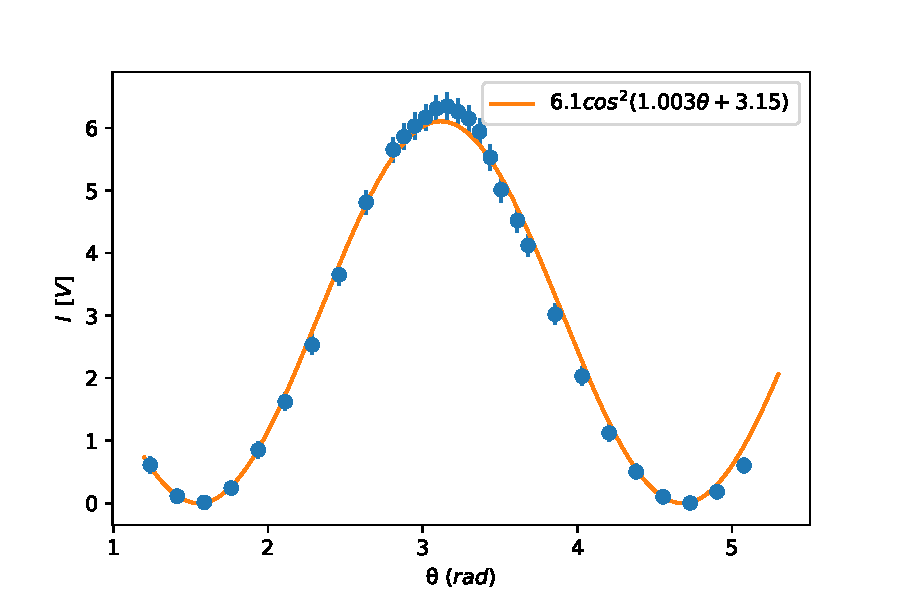
\includegraphics[width=\linewidth]{malus1.pdf}
	\captionof{figure}{\small{Voltaggio ai capi del fotodiodo in funzione dell'angolo di rotazione $\theta$ tra i due assi di polarizzazione dei filtri.Ai dati è sovrapposta la curva teorica con i parametri di fit.}}
	\label{fig:malus}
	\end{center}
\end{Figure}

\section{Angolo di Brewster}
Si monta l'apparato in Figura \ref{opt:brewster}, dove prima del fotodiodo è stato posizionato un \emph{beamsplitter polarizzatore}, in grado di trasmettere la componente orizzontale o quella verticale\footnote{Quale delle due componenti viene trasmessa e quale riflessa dipende da come è costruito e come è montato il beamsplitter.} della radiazione e riflettere la componente ortogonale, con coefficiente di assorbimento complessivo quasi nullo. 

Posizionando tra il beamsplitter e il rilevatore un dielettrico (perspex) in modo che il piano di incidenza del laser fosse parallelo al piano di lavoro, si è ottenuto che la componente verticale della radiazione coincidesse con la componente TE e quella orizzontale con la TM.

Per capire quale delle due componenti veniva trasmessa dal beamsplitter, lo si è posizionato tra il filtro polarizzatore e il dielettrico e si è controllato visivamente il raggio riflesso al variare dell'angolo di incidenza: nel nostro caso si è visto che il riflesso si annullava per un angolo particolare (quello di Brewster, appunto), dunque abbiamo dedotto che la componente trasmessa fosse quella orizzontale, cioè di tipo TM.

Si è dunque rimosso il dielettrico e si è visto per quale angolo del polarizzatore la componente riflessa si annullava: nel nostro caso specifico si è misurato un angolo $\theta_{\mathrm{TM}} = \SI{52 \pm 1}{°}$ per cui tutto il laser veniva trasmesso, quest'angolo corrisponde ad una direzione verticale dell'asse di trasmissione del polarizzatore. Si è dunque verificato che a $\theta_{\mathrm{TE}} = \theta_{\mathrm{TM}} - \SI{90}{°} = \SI{322 \pm 1}{°}$ la componente trasmessa si annullasse, allora $\theta_{\mathrm{TE}}$ corrisponde all'asse di trasmissione in direzione orizzontale.

Misurate le posizioni del polarizzatore corrispondenti alle due componenti di interesse, si è rimosso il beamsplitter dall'apparato e si è cominciato a prendere misure di intensità del raggio riflesso dal dielettrico al variare dell'angolo di incidenza. Nel fare questo si è tenuto conto che l'intensità del laser diminuisce all'aumentare della distanza dalla sorgente a causa di fenomeni diffrattivi, quindi si è cercato di mantenere il rilevatore sempre alla stessa distanza dal dielettrico.

Inoltre bisogna tener conto del fatto che i raggi riflessi dal dielettrico sono due: quello riflesso dalla prima superficie e quello riflesso dalla seconda. Nel fare la misura bisogna considerare che il raggio di interesse è quello corrispondente alla riflessione sulla prima superficie, riconoscibile perché associato all'angolo di riflessione minore.

Per ogni angolo di incidenza, fissato il rilevatore in modo che il fotodiodo misurasse l'intensità maggiore, si è misurata l'intensità per entrambe le componenti, ruotando il polaroid e posizionandolo sugli angoli $\theta_{\mathrm{TE}}$ e $\theta_{\mathrm{TM}}$ misurati in precedenza.

\subsection{Riflettanza}
Gli andamenti previsti per le riflettanze, ovvero i rapporti tra l'intensità misurata e quella misurata in assenza di dielettrico, sono descritti dalle due curve
\begin{equation}\label{eq:rs}
	r_{\mathrm{TE}} = r_ s = \frac{\cos \theta - \sqrt{n^2 - \sin^2 \theta}}{\cos \theta + \sqrt{n^2 - \sin^2 \theta}},
\end{equation}
\begin{equation}\label{eq:rs}
	r_{\mathrm{TE}} = r_p =  \frac{-n^2 \cos \theta + \sqrt{n^2 - \sin^2 \theta}}{n^2 \cos \theta + \sqrt{n^2 - \sin^2 \theta}},
\end{equation}
dove $n$ è il rapporto tra l'indice di rifrazione del dielettrico e quello dell'aria.
Il risultato della misura è riportato in Figura \ref{fig:brewster_I}, dove ai dati sperimentali sono sovrapposte le curve teoriche corrispondenti a $n_s = \SI{1.49 \pm 0.01}{}$ e $n_p = \SI{1.50 \pm 0.02}{}$, valori ottenuti fittando le curve sui dati sperimentali.
\begin{Figure}
	\begin{center}
	\includegraphics[width=\linewidth]{riflettanze.pdf}
	\captionof{figure}{Riflettanza delle componenti TE e TM al variare dell'angolo di incidenza, si riportano le curve teoriche fittate.}
	\label{fig:brewster_I}
	\end{center}
\end{Figure}

\subsection{Visibilità}
Per stimare l'angolo di Brewster del dielettrico, ossia l'angolo per cui l'intensità della componente TM del fascio riflesso si annulla, si studia la visibilità del fascio definita come
\begin{equation}\label{eq:visibilità}
	V(\theta) = \frac{r_s(\theta) - r_p(\theta)}{r_s(\theta) + r_p(\theta)}
\end{equation}
dalla cui definizione è evidente che
\begin{equation}
	\left. V(\theta) \right\vert_{\theta = \theta_\mathrm{Brewster}} = 1.
\end{equation}
In Figura \ref{fig:brewster_V} sono riportati i dati sperimentali insieme alla curva teorica corrispondente a $n_V = \SI{1.61 \pm 0.04}{}$, ottenuto fittando i dati.
\begin{Figure}
	\begin{center}
	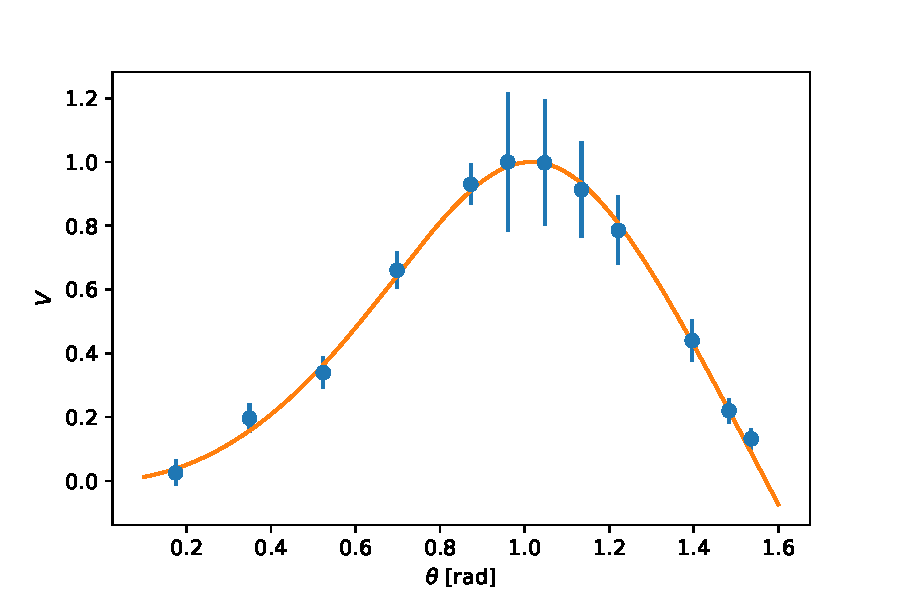
\includegraphics[width=\linewidth]{visibilità.pdf}
	\captionof{figure}{Visibilità del raggio riflesso, si riporta la curva teorica fittata.}
	\label{fig:brewster_V}
	\end{center}
\end{Figure}
Si nota che i diversi valori di $n$ ottenuti in quest'ultima parte dell'esperienza sono incompatibili tra loro, ciò è sintomo di una sottostima delle incertezze sui valori di intensità.
Per stimare l'angolo $\theta_\mathrm{max}$ corrispondente al massimo della visibilità, si fa una media trai due angoli corrispondenti ai valori misurati della visibilità più alti, si ottiene
\begin{equation}
	\theta_\mathrm{max} = \theta_\mathrm{brewster} = \SI{57 \pm 2}{°}
\end{equation}
da cui, essendo 
\begin{equation}
	\theta_\mathrm{brewster} = \arctan (n)
\end{equation}
si trova 
\begin{equation}
	n = \tan (\theta_\mathrm{brewster} )= \SI{1.54 \pm 0.05}{},
\end{equation}
compatibile con i valori ottenuti precedentemente.

\end{multicols}


\end{document}
